\chapter{Finance}
The finances for Venturer Camp 2023 were overseen by the Head of Resources at Woodcraft Folk with assistance and knowledge given from the Venturer Camp Treasurer and Coordinator. The decision to manage the finances like this came about from not having anyone in the treasurer post at the start of the project so the Coordinator and HoR began managing the finances themselves, then once a treasurer was appointed this felt like the simplest option. \\

The management of finances through the Woodcraft Folk systems had a number of benefits and drawbacks. The most notable benefit was that it was all dealt with for us (``us'' being the Core Team), with trained professionals managing the day to day running of the finance. The Treasurer was able to support by approving expenses and invoice payments as well as doing the first level of chasing for payments, later levels of chasing were done by the HoR.\\

One of the significant drawbacks of using the very established Woodcraft Folk finance system is that it is already set up very firmly. The Venturer Camp team's budget lines didn't match the central monitoring system, and this made our lives much more difficult when reviewing payments into and out of the account in order to monitor how much was being spent in each category. This was further exacerbated by the fact that the finance monitoring tools (a series of Google Sheets) were set up such that they required a great level of understanding to be able to read them. This resulted in large amounts of confusion amongst those people who had to read them and understand them. \\

Another significant drawback of using the Woodcraft Folk finance system was that quite often transactions were ``mis-coded'' within the system. This resulted in transactions erroneously appearing on the monitoring spreadsheet, or not appearing altogether - leading us to believe we hadn't spent as much as we in fact had. 

\section{Budget}
The first budget for Venturer Camp 2023 was drawn up by Woodcraft's Chief Executive using figures from Venturer Camp 2019 and Common Ground International Camp 2022 to influence expected expenditure for 2023. Throughout the project, minor alterations were made to the budget, mostly to reflect the change in expected income due to fundraising income being lower than initially expected.\\

Due to the above mentioned issues with the coding of income and expenditure within the Woodcraft Folk finance systems, and the fact that they do not line up with our budget lines - we do not have a final breakdown of expected vs actual for our budget.\\

Shown below is the Venturer Camp 2023 budget, compared to the Venturer Camp 2019 actual expenditure. 

{\RaggedRight \centering
    \begin{longtable}{p{0.5\textwidth} p{0.2\textwidth} p{0.2\textwidth}}
    \textbf{Category} & \textbf{2019 Actual} & \textbf{2023 Budget}\\
    \hline
    \hline
    \endhead

    \multicolumn{3}{r}{\footnotesize\itshape continued on next page}\\
    \endfoot 

    \endlastfoot

    Number of paying campers & ? & 300\\
    \hline
    Number of campers & 434 & 400\\
    \hline
    Price per camper & 125/135/150 & 150\\
    \hline
    \multicolumn{1}{r}{\textit{Total Camp Fees}} & 52411 & 45000\\
    \hline
    \multicolumn{3}{l}{\textbf{Other Income}}\\
    \hline
    Pre-Camp Food Contribution & & 750\\
    \hline
    Christmas Challenge Access Fund & 0 & 5000\\
    \hline
    Merchandise Sales & ? & 1800\\
    \hline
    Restricted Fundraising & ? & 6000\\
    \hline
    Unrestricted Fundraising & ? & 4000\\
    \hline
    \rowcolor{accent!60}
    \multicolumn{1}{r}{\textit{Total Income}} & & 62550\\
    \hline

    \caption{Venturer Camp 2023 Income Budget}
    \end{longtable}
} % end of rr  


{\RaggedRight \centering
    \begin{longtable}{p{0.5\textwidth} p{0.2\textwidth} p{0.2\textwidth}}
    \textbf{Category} & \textbf{2019 Actual} & \textbf{2023 Budget}\\
    \hline
    \hline
    \endhead

    \multicolumn{3}{r}{\footnotesize\itshape continued on next page}\\
    \endfoot 

    \endlastfoot

    Site Fees & 10500 & 15000\\
    \hline
    Food & 10811 & 14000\\
    \hline
    Pre-Camp food \& pitch (50 people max) & & 1300\\
    \hline
    Evening Programme & 1830 & 1750 \\
    \hline
    Day Programme & 1599 & 1500\\
    \hline
    Adventurous Activities & 0 & 4000\\
    \hline
    Printed Material & 140 & 450 \\
    \hline
    T-Shirts & 240 & 0\\
    \hline
    Merchandise & 0 & 1500\\
    \hline
    Website & 72 & 50 \\
    \hline
    Wristbands & 400 & 450 \\
    \hline
    Toilet Hire & 600 & 750\\
    \hline
    Fridge Hire & ? & 1750 \\
    \hline
    PA, Stage \& Lighting Hire & 1000 & 800\\
    \hline
    Coach Hire for Shuttle Service & ? & 2500\\
    \hline
    Main Marquee Hire & 7000 & 6000\\
    \hline
    Village Equipment Transport Van Hire & ? & 2800\\
    \hline
    Volunteer Expenses & 2466 & 2000\\
    \hline
    Tables \& Chairs & 1500 & 1500\\
    \hline
    Contingency & ? & 6000\\
    \hline
    Contribution to Core & 5000 & 0 \\
    \hline
    Venturer Committee & 6000 & 0\\
    \hline
    \rowcolor{accent!60}
    \multicolumn{1}{r}{\textit{Total Expenditure}} & 49158 & 64100\\
    \hline

    \caption{Venturer Camp 2023 Expenditure Budget}
    \end{longtable}
} % end of rr  


Broadly speaking, there was enough money in each budget category for the expenditure required. The only places where we felt the strain was within the \textit{PA, Stage and Lighting} hire where the stage hire came out as nearly \pounds2k where we had only budgeted \pounds800.\\

There were some other expenditures which were higher than originally anticipated, relating to the Solar Array configuration - the difference here was absorbed through a combination of reducing Programme budget and volunteers buying-back the equipment from Woodcraft Folk after the event.\\

The budget was designed with rental fees for a trailer refrigeration unit in mind. Due to not being able to power a unit like this, the majority of this budget line was re-allocated to the other budget categories, such as Solar equipment. The lack of adequate refrigeration was something which caused the food team many difficulties and is something which should be carefully considered at future events.

\section{Outgoing Payments}
\subsection{Ahead of Camp}
Woodcraft Folk aim to reduce the admin taken to expensing people as much as possible. To help with this, payments should be and generally were made by invoice to Woodcraft Folk where possible. This can be done with a form that Woodcraft Folk staff have access to, and the coordinator and treasurer should be given access too. \\
The deadline for the weekly payment run is Tuesday, so  forms should be submitted by then in order for the Finance staff to have time to process payment by the end of the week. If we need urgent invoice payments, this is also possible by talking to the finance team.\\ 

For things that can only be bought on card, this was done via the Events Assistant, Programmes Manager or CEO where possible, as they all have Woodcraft Folk credit cards and this means Woodcraft Folk are charged directly and there is no need for anyone to be out of pocket.\\

Discussions were had surrounding the use of prepaid cards for certain teams. It was agreed that these would be sensible to attempt to get however due to complications (i.e. time pressures, exams, not having obvious people to give a card), we were unable to follow through with this. We would recommend this in future so it is easier for essential last minute payments to be made by budget holders (e.g the food and programme teams) in the final month leading up to camp and on site. Being able to pay by card directly and not have to organise doing so with a staff member would reduce admin for volunteer budget holders as well as staff members.

\subsection{On-Camp}
On camp, sometimes people need to buy things urgently e.g food items that haven't been delivered, equipment for programme that is missing, items to repair tents or other equipment in case of unusual weather conditions etc. Often these will be things we cannot get from suppliers we have accounts with due to availability of the items/how urgently we need them.\\

This camp we managed to minimise the number of volunteers out of pocket/the admin taken to expense them as we had 3 members of staff on site with Woodcraft Folk credit cards. The food team took the CEO's credit card off site to buy emergency items on a few occasions, and the Events Assistant also ordered some things to be delivered to site the next day on her credit card.\\

Volunteers also ordered some things on their personal bank cards which were reimbursed. We looked to minimise the spread of this as far as possible, with the Coordinator and other central volunteers ordering the majority, rather than the wider volunteer team being expected to do this.

\section{Expenses}
Through utilising the Woodcraft Folk finance system, we had access to an already well-established expenses procedure which many volunteers were already familiar with from other events.\\

Core volunteers were able to either put their own expenses through a Google Form, or have the treasurer put them through for them. The treasurer would then have to approve every individual expense request before it went to the Finance Team to be paid. This system worked for the most part as we were clear about what could \& couldn't be expensed apart from one incident.\\

The only incident surrounding expenses was where communications were had with a young person rather than their parent who was driving them to \& from the camp. This caused some confusion around what legs of their journey could legitimately be claimed for and what couldn't; when all other members of the team weren't able to claim for their personal journeys to \& from the main camp as we simply didn't have the budget to stretch this for everyone.\\

For clarity in the future, it might be advisable to only allow the treasurer to put in expenses claims, requiring a coordinator to sign off on them. This is a conversation that should be had between the HoR, Camp Coordinator \& Treasurer to ensure everyone is on the same page and the systems are set up correctly.

\section{Supplier Accounts}
\subsection{Food Accounts}
The Head of Resources helped lots with setting up accounts with food suppliers. He did the forms they asked for with proof of finances etc, and set up a Woodcraft Folk email for contacting suppliers/accessing accounts with them so we could use that for all events in future rather than changing the contact details all the time.\\

We already had an account with Booker; which the Chief Executive is responsible for the upkeep of, including changing our `home branch' for the duration of events. Additionally, supplier accounts were created with: Evans and Castell Howell.

\subsection{Equipment Suppliers}
Woodcraft Folk have an account with Viking. We ordered some stationary, cleaning and generic Site Services supplies through them. They are cheap and good for bulk orders in advance of camp. The delivery gets delivered directly to the site which aids transport logistics massively! The SMT Assistant on the Woodcraft Folk staff team is the only person who can make orders to this company, which adds a little bit of processing time - however we knew about this far enough in advance for it not to cause an issue.\\

For programme specific resources, and general stationery supplies, we used Manchester Woodcraft Folk's YPO account. The suggestion to use this came from the Head of Memberships \& Programmes who is a leader in Manchester. This worked very well and was cheaper than Viking for stationary and other programme supplies. Woodcraft Folk should look into registering as a central unit for this for future events. 

\section{Access Fund}
At the time of project initiation, and then while discussing ticket prices, it was decided that an access fund should be created. This would aim to support disadvantaged Young People and Adults to attend camp as participants and volunteers respectively.\\

To apply for the access fund, there was a short form which allowed the applicant to self indicate their responses to the following questions:
\begin{itemize}
    \item I am eligible for Free School Meals
    \item I am in receipt of Universal Credit
    \item I would describe myself as disabled
    \item I would describe myself as a person of colour
\end{itemize}
The responses to this form were then analysed, in combination with the applicant's distance from Biblins, to distribute the funds. Discounts were applied to bookings where an individual had received some money from the access fund.\\

This worked successfully, especially to support some of the larger groups who were travelling via group-hired coaches, engaging more people in Venturer Camp than we would otherwise have expected.\\

The access fund was publicised through our website, emails to group leaders and social media.

\section{Fundraising}
We had planned to raise a considerable amount of our income through fundraising activity as this would further reduce the ticket price therefore enabling more young people to attend the event. Unfortunately, we were unable to find suitable grants which we could apply for, and therefore unable to meet our fundraising target.\\

We were successfully able to raise some funds through fundraising, mostly from a sponsored event in which three DFs coracled \& kayaked down the Wye. 
\begin{figure}[ht]
    \centering
    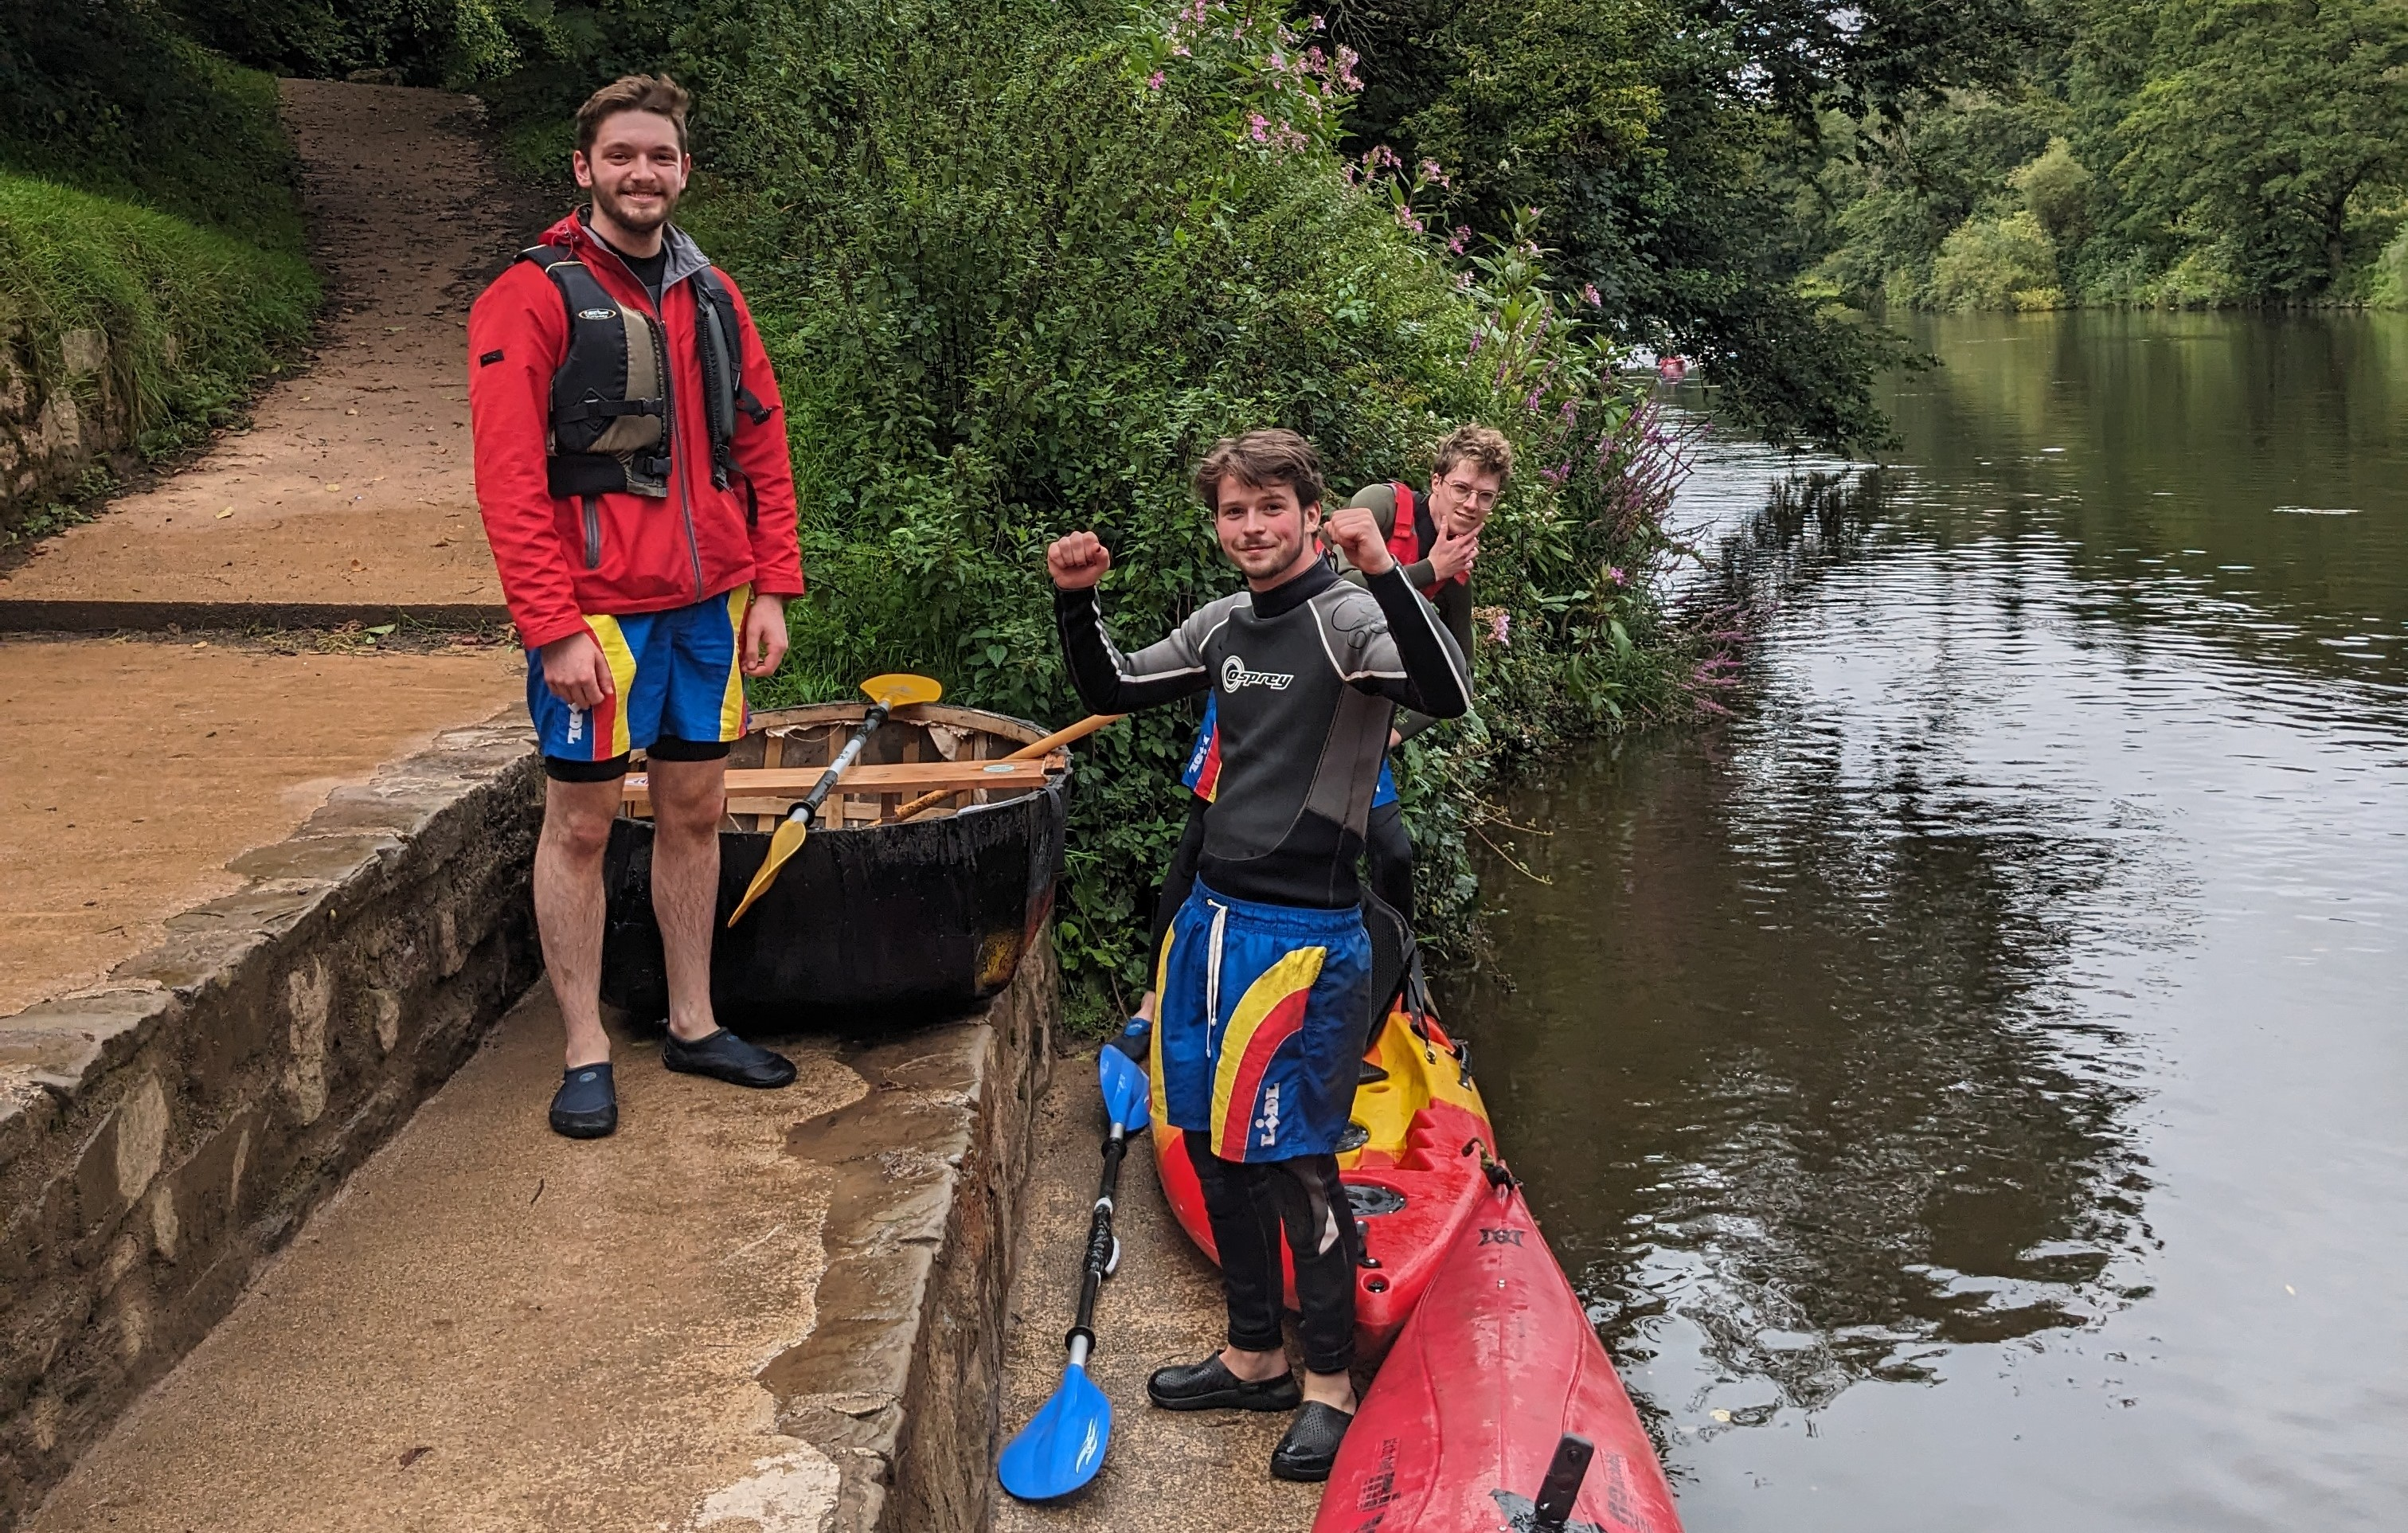
\includegraphics[width=0.8\textwidth]{assets/coracle-team.jpg}
    \caption{Coracle fundraising team back on dry land (\textit{TB})}
\end{figure}

\section{VCoin}
Due to the lack of signal at Biblins Campsite and the desire to minimise cash handling from the Woodcraft Folk Finance Team - it was decided to use an on-camp currency. This would solve our problem of wanting people to pay by card and only having one location on site where we could use a card machine.\\

The currency used, deemed ``VCoin'' was represented by poker chips which were sourced from a Member of Staff's local Rotary Club. These worked out very well for us as there was a plentiful supply of them in not-too-awkward denominations which we weren't charged for the hire of.\\

The currency exchange rate was 1:1. Attendees were able to exchange as much GBP to VCoin as they wished, however only values over \pounds5 would be returned to GBP at the end of camp. This was due to the fact that we didn't have capacity to handle high amounts of cash. This decision was frowned upon by many and for future events where there is a requirement to use an on-camp currency - it would be suggested to increase capacity for refunds at the end of the event.\\

The use of the currency on site caused lots of difficulties. It had originally been planned that the bank would only be open for a few hours a day; it was very quickly learnt however that Venturers aren't that organised and the bank had to be open at any time money could be spent (i.e. whenever the shop or cafe was open). This caused staffing issues for the bank as it had only been planned for the Treasurer to staff the bank, whereas we had to source more volunteers to staff it while the Treasurer was handling other finance related duties. The Cafe team in particular noted that not having the bank open at the times they were open led to a loss in sales, where an attendee would wish to purchase something but wouldn't be able to due to not having any VCoin and the bank wasn't open. \\

For future events which require the use of an on-camp currency, it would be suggested to: define the opening hours for the bank further in advance; ensure that any time money can be spent on site; better plan for the end of the camp where more provision should be looked for to exchange the camp currency back to GBP. 

\section{Final report \& Figures as at 1 November 2023}
The original budget assumed Venturer Camp would break even but make no contribution to overhead costs. The Final Forecast recognised attendance and income were lower than originally planned. While attempts were made to reduce expenditure to offset the reduction on income it was recognised it would be challenging to retain a breakeven position and the final forecast assumed a \pounds4k deficit. The final position presents a \pounds2k deficit.\\

Income was \pounds6k (10\%) lower than originally planned due to lower levels of attendance.\\

Expenditure was \pounds8k (12\%) lower than the final forecast and \pounds4k lower than the original budget. All areas of expenditure finished very close to budget with the only material underspends relating to `Other' (\pounds7k) which included a \pounds4k contingency for the potential reduction in income. `Total Premises' finished \pounds21k underspent, however, this is offset with the `Internal Centre Fees'overspend (\pounds19.4k) which relates to the internal transfer of funds to Biblins for the hire of the site.

{\RaggedRight \centering
    \begin{longtable}{p{0.3\textwidth} p{0.1\textwidth} p{0.13\textwidth} p{0.1\textwidth} p{0.1\textwidth} p{0.1\textwidth}}
    \textbf{} & \textbf{2023 Actual} & \textbf{2023 Final Forecast} & \textbf{Variance} & \textbf{Variance (\%)} & \textbf{2023 Budget}\\
    \hline
    \hline
    \endhead

    \multicolumn{6}{r}{\footnotesize\itshape continued on next page}\\
    \endfoot 

    \endlastfoot

    \multicolumn{6}{l}{\textbf{External Income}}\\*
    Events & 44,109 & 45000 & -891 & -2\% & 45000\\*
    Donations & 165 & 5,750 & -5,585 & -97\% & 5,750 \\*
    Restricted Grant & 0 & 6,000 & -6,000 & -100\% & 6,000 \\*
    Unrestricted Grant & 0 & 4,000 & -4,000 & -100\% & 4,000 \\*
    Stock Sales & 4,690 & 1,250 & 3,440 & 275\% & 1,250 \\*
    Internal Events & 1,851 & 0 & 1,851 & 0\% & 0\\*
    \multicolumn{1}{r}{\textit{Total External Income}} & 50,815 & 62,000 & -11,185 & -18\% & 62,000\\
    \hline
    \multicolumn{6}{l}{\textbf{Internal Income}}\\*
    Internal Transfers & 5,250 & 0 & 5,250 & 0\% & 0\\*
    \multicolumn{1}{r}{\textit{Total External Income}}& 5,250 & 0 & 5,250 & 0\% & 0\\*
    \hline
    \rowcolor{accent!60}
    \multicolumn{1}{r}{\textit{Total Income}}& 56,065 & 62,000 & -5,935 & -10\% & 62,000\\
    \hline
    \multicolumn{6}{l}{\textbf{People}}\\*
    Travel \& Subsistence & 2,120 & 2,000 & 120 & 6\% & 2,000\\*
    \multicolumn{1}{r}{\textit{Total People}} & 2,120 & 2,000 & 120 & 6\% & 2,000\\*
    \hline
    \multicolumn{6}{l}{\textbf{Direct Costs of Sale}}\\*
    Activities Expenditure & 24,033 & 7,250 & 16,783 & 231\% & 7,250 \\*
    Catering Expenditure & 661 & 15,300 & -14,639 & -96\% & 15,300 \\*
    Cost of Sales & 0 & 1,500 & -1,500 & -100\% & 1,500 \\*
    \multicolumn{1}{r}{\textit{Total Direct Costs of Sale}} & 24,695 & 24,050 & 645 & 3\% & 24,050 \\
    \hline
    \multicolumn{6}{l}{\textbf{Premises}}\\*
    Gas & 855 & 0 & 855 & 0\% & 0 \\*
    Other Utilities & 145 & 0 & 145 & 0\% & 0 \\*
    Rent \& Rates & 0 & 15,000 & -15,000 & -100\% & 15,000 \\*
    Cleaning & 17 & 0 & 17 & 0\% & 0 \\*
    Equipment & 6,710 & 13,936 & -7,226 & -52\% & 13,936 \\*
    \multicolumn{1}{r}{\textit{Total Premises}} & 7,727 & 28,936 & -21,209 & -73\% & 28,936\\
    \hline
    \multicolumn{6}{l}{\textbf{Other}}\\*
    Fundraising and Marketing & 3,217 & 0 & 3,217 & 0\% & 0 \\*
    Administration & 865 & 0 & 865 & 0\% & 0 \\*
    Other & 0 & 11,014 & -11,014 & -100\% & 7,014 \\*
    Bad Debt & 0 & 0 & 0 & 0\% & 0 \\*
    \multicolumn{1}{r}{\textit{Total Other}} & 4,082 & 11,014 & -6,932 & -63\% 0 & 7,014 \\
    \hline
    \multicolumn{6}{l}{\textbf{Internal}}\\*
    Internal Centre Fees E & 19,442 & 0 & 19,442 & 0\% & 0 \\*
    \multicolumn{1}{r}{\textit{Total Internal}} & 19,442 & 0 & 19,442 & 0\% & 0 \\*
    \hline
    \rowcolor{accent!60}
    \multicolumn{1}{r}{\textit{Total Expenditure}} & 58,066 & 66,000 & -7,934 & -12\% & 62,000 \\
    \hline
    \hline
    \rowcolor{accent!60}
    \multicolumn{1}{r}{\textbf{Annual Surplus/(Deficit)}} & -2,001 & -4,000 &  &  & 0 \\
    \hline

    \caption{Venturer Camp 2023 Final Figures}
    \end{longtable}
} % end of rr 